% TikZ schematics as people draw them in talks, one way of drawing per frame, from the plain box
% and arrow that already becomes native shapes to the ones that still stay pictures (curved
% edges, edge labels, math labels, containers, shadows, shadings, multipart nodes, circuits).
% The frame title names what the frame tries; keep one new thing per frame so a refusal points
% at its cause.
\documentclass{beamer}
\usepackage{tikz}
\usetikzlibrary{arrows.meta, positioning, calc, fit, backgrounds, shapes.geometric,
  shapes.multipart, shapes.symbols, shapes.misc, automata, matrix, trees, mindmap, shadows,
  decorations.pathreplacing, chains}
\usepackage{tikz-cd}
\usepackage[siunitx]{circuitikz}
\title{TikZ diagrams}
\author{Tester}
\date{}

\tikzset{
  box/.style={draw, rounded corners=2pt, fill=blue!10, minimum height=0.8cm, minimum width=1.8cm},
  sq/.style={draw, fill=orange!15, minimum height=0.8cm, minimum width=1.8cm},
  arr/.style={-{Stealth[length=2.5mm]}, thick},
  layer/.style={draw, fill=#1, minimum width=7cm, minimum height=0.8cm},
}

\begin{document}

% --- Baseline: what becomes native today ------------------------------------------------------

\begin{frame}{Straight pipeline}
  \centering
  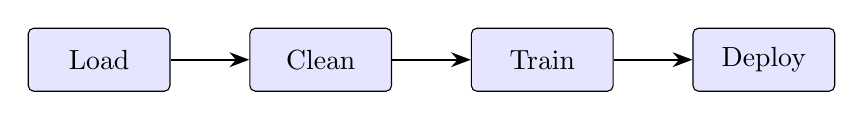
\begin{tikzpicture}[node distance=1cm]
    \node[box] (a) {Load};
    \node[box, right=of a] (b) {Clean};
    \node[box, right=of b] (c) {Train};
    \node[box, right=of c] (d) {Deploy};
    \draw[arr] (a) -- (b);
    \draw[arr] (b) -- (c);
    \draw[arr] (c) -- (d);
  \end{tikzpicture}
\end{frame}

\begin{frame}{Flowchart with a decision and a loop back}
  \centering
  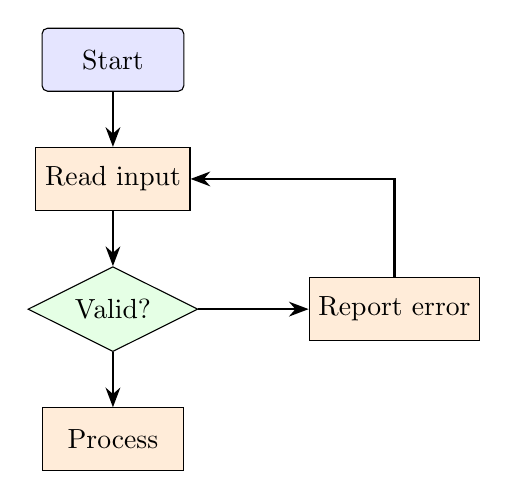
\begin{tikzpicture}[node distance=0.7cm and 1.4cm]
    \node[box] (start) {Start};
    \node[sq, below=of start] (read) {Read input};
    \node[draw, diamond, aspect=2, fill=green!10, below=of read] (ok) {Valid?};
    \node[sq, below=of ok] (go) {Process};
    \node[sq, right=of ok] (err) {Report error};
    \draw[arr] (start) -- (read);
    \draw[arr] (read) -- (ok);
    \draw[arr] (ok) -- (go);
    \draw[arr] (ok) -- (err);
    \draw[arr] (err) |- (read);
  \end{tikzpicture}
\end{frame}

% --- Edges ------------------------------------------------------------------------------------

\begin{frame}{Edge labels above and below the arrows}
  \centering
  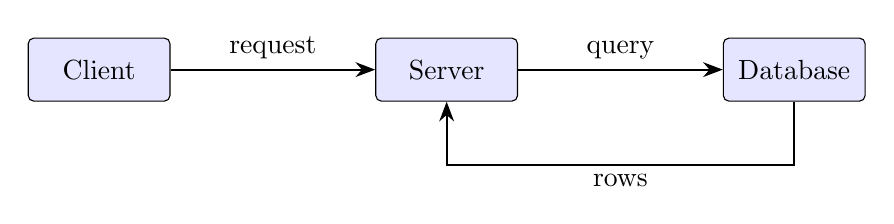
\begin{tikzpicture}[node distance=2.6cm]
    \node[box] (c) {Client};
    \node[box, right=of c] (s) {Server};
    \node[box, right=of s] (db) {Database};
    \draw[arr] (c) -- node[above] {request} (s);
    \draw[arr] (s) -- node[above] {query} (db);
    \draw[arr] (db.south) -- ++(0,-0.8) -| node[pos=0.25, below] {rows} (s.south);
  \end{tikzpicture}
\end{frame}

\begin{frame}{Curved edges: bend left and bend right}
  \centering
  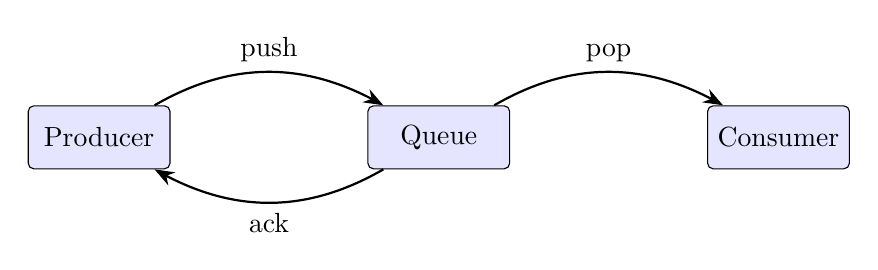
\begin{tikzpicture}[node distance=2.5cm]
    \node[box] (a) {Producer};
    \node[box, right=of a] (b) {Queue};
    \node[box, right=of b] (c) {Consumer};
    \draw[arr] (a) to[bend left] node[above] {push} (b);
    \draw[arr] (b) to[bend left] node[below] {ack} (a);
    \draw[arr] (b) to[bend left] node[above] {pop} (c);
  \end{tikzpicture}
\end{frame}

\begin{frame}{Edges with out and in angles}
  \centering
  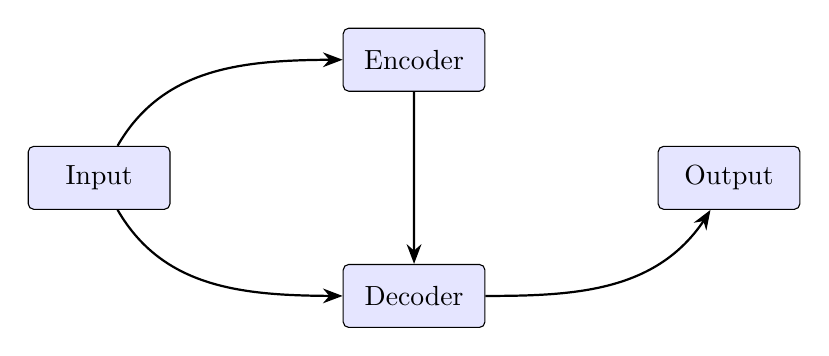
\begin{tikzpicture}
    \node[box] (a) at (0,0) {Input};
    \node[box] (b) at (4,1.5) {Encoder};
    \node[box] (c) at (4,-1.5) {Decoder};
    \node[box] (d) at (8,0) {Output};
    \draw[arr] (a) to[out=60, in=180] (b);
    \draw[arr] (b) to[out=-90, in=90] (c);
    \draw[arr] (c) to[out=0, in=-120] (d);
    \draw[arr] (a) to[out=-60, in=180] (c);
  \end{tikzpicture}
\end{frame}

\begin{frame}{Dashed and dotted edges}
  \centering
  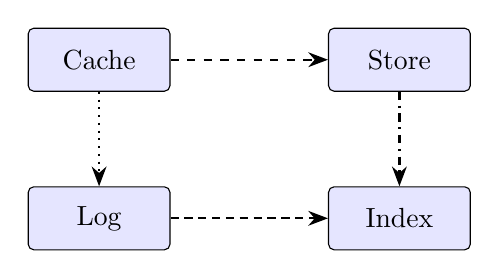
\begin{tikzpicture}[node distance=1.2cm and 2cm]
    \node[box] (a) {Cache};
    \node[box, right=of a] (b) {Store};
    \node[box, below=of a] (c) {Log};
    \node[box, below=of b] (d) {Index};
    \draw[arr, dashed] (a) -- (b);
    \draw[arr, dotted] (a) -- (c);
    \draw[arr, dash dot] (b) -- (d);
    \draw[arr, densely dashed] (c) -- (d);
  \end{tikzpicture}
\end{frame}

\begin{frame}{Arrow tips: double, Latex, circle, bar}
  \centering
  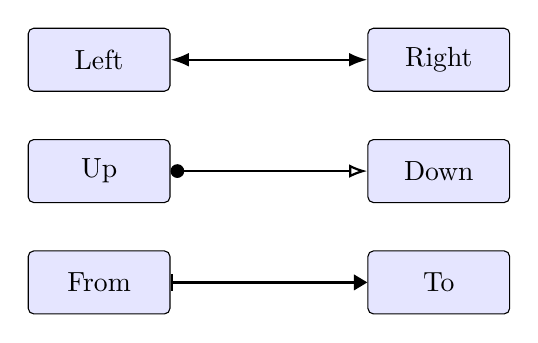
\begin{tikzpicture}[node distance=0.6cm and 2.5cm]
    \node[box] (a) {Left};
    \node[box, right=of a] (b) {Right};
    \node[box, below=of a] (c) {Up};
    \node[box, right=of c] (d) {Down};
    \node[box, below=of c] (e) {From};
    \node[box, right=of e] (f) {To};
    \draw[{Latex}-{Latex}, thick] (a) -- (b);
    \draw[{Circle}-{Latex[open]}, thick] (c) -- (d);
    \draw[{Bar}-{Triangle}, thick] (e) -- (f);
  \end{tikzpicture}
\end{frame}

\begin{frame}{Self loops and parallel edges}
  \centering
  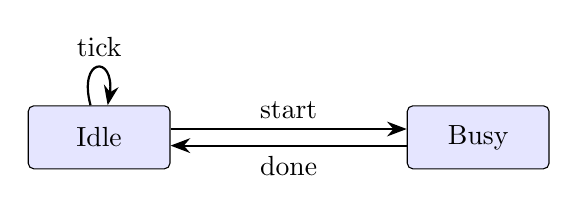
\begin{tikzpicture}[node distance=3cm]
    \node[box] (a) {Idle};
    \node[box, right=of a] (b) {Busy};
    \draw[arr] (a) to[loop above] node[above] {tick} (a);
    \draw[arr] ([yshift=3pt]a.east) -- node[above] {start} ([yshift=3pt]b.west);
    \draw[arr] ([yshift=-3pt]b.west) -- node[below] {done} ([yshift=-3pt]a.east);
  \end{tikzpicture}
\end{frame}

\begin{frame}{Sloped labels along diagonal edges}
  \centering
  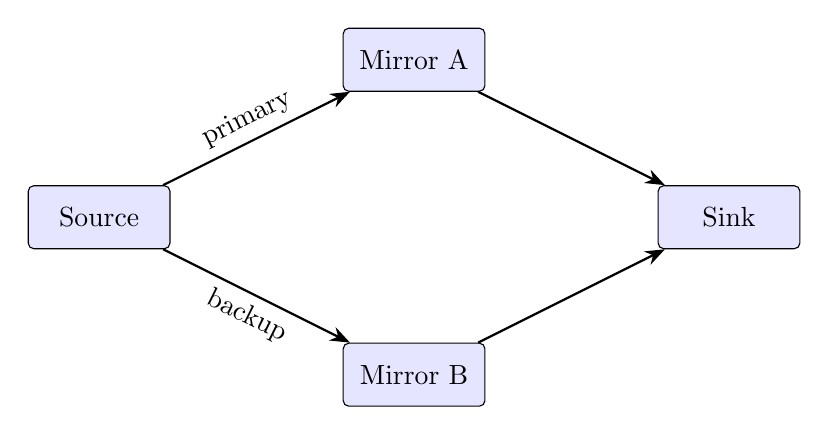
\begin{tikzpicture}
    \node[box] (a) at (0,0) {Source};
    \node[box] (b) at (4,2) {Mirror A};
    \node[box] (c) at (4,-2) {Mirror B};
    \node[box] (d) at (8,0) {Sink};
    \draw[arr] (a) -- node[above, sloped] {primary} (b);
    \draw[arr] (a) -- node[below, sloped] {backup} (c);
    \draw[arr] (b) -- (d);
    \draw[arr] (c) -- (d);
  \end{tikzpicture}
\end{frame}

% --- Nodes ------------------------------------------------------------------------------------

\begin{frame}{Multi-line node text}
  \centering
  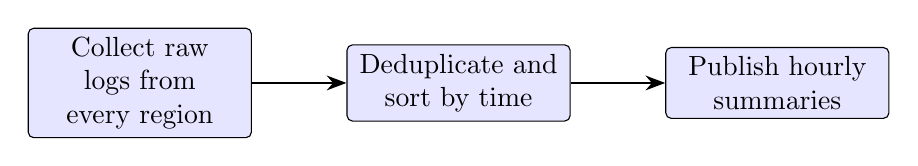
\begin{tikzpicture}[node distance=1.2cm,
      wide/.style={box, text width=2.6cm, align=center}]
    \node[wide] (a) {Collect raw logs from every region};
    \node[wide, right=of a] (b) {Deduplicate and sort by time};
    \node[wide, right=of b] (c) {Publish hourly summaries};
    \draw[arr] (a) -- (b);
    \draw[arr] (b) -- (c);
  \end{tikzpicture}
\end{frame}

\begin{frame}{Shapes: cylinder, ellipse, hexagon, circle}
  \centering
  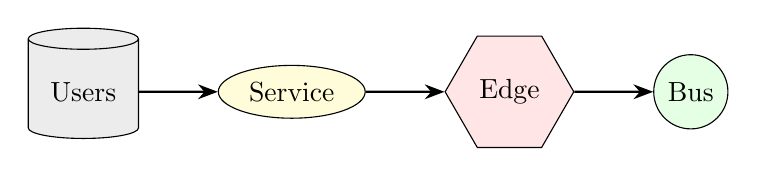
\begin{tikzpicture}[node distance=1cm]
    \node[draw, cylinder, shape border rotate=90, aspect=0.25, fill=gray!15, minimum height=1.4cm,
      minimum width=1.4cm] (db) {Users};
    \node[draw, ellipse, fill=yellow!15, right=of db] (e) {Service};
    \node[draw, regular polygon, regular polygon sides=6, fill=red!10, right=of e] (h) {Edge};
    \node[draw, circle, fill=green!10, right=of h] (c) {Bus};
    \draw[arr] (db) -- (e);
    \draw[arr] (e) -- (h);
    \draw[arr] (h) -- (c);
  \end{tikzpicture}
\end{frame}

\begin{frame}{Shapes: cloud, document, chamfered, pill}
  \centering
  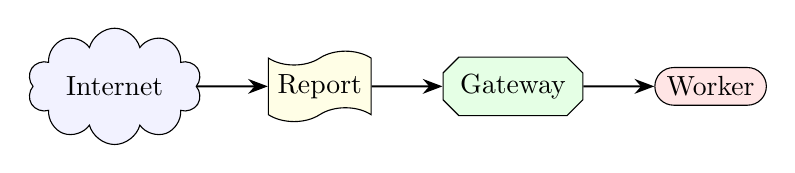
\begin{tikzpicture}[node distance=0.9cm]
    \node[draw, cloud, cloud puffs=10, aspect=2, fill=blue!5] (cl) {Internet};
    \node[draw, tape, fill=yellow!10, right=of cl] (doc) {Report};
    \node[draw, chamfered rectangle, fill=green!10, right=of doc] (ch) {Gateway};
    \node[draw, rounded rectangle, fill=red!10, right=of ch] (p) {Worker};
    \draw[arr] (cl) -- (doc);
    \draw[arr] (doc) -- (ch);
    \draw[arr] (ch) -- (p);
  \end{tikzpicture}
\end{frame}

\begin{frame}{Rotated ellipse and rotated rectangle}
  \centering
  
\begin{tikzpicture}
    \node[draw, ellipse, fill=blue!10, rotate=30, minimum width=2.5cm] (a) at (0,0) {Orbit};
    \node[draw, fill=orange!15, rotate=-20, minimum width=2cm] (b) at (5,0) {Tilted};
    \draw[arr] (a) -- (b);
  \end{tikzpicture}
\end{frame}

\begin{frame}{UML class: a multipart node}
  \centering
  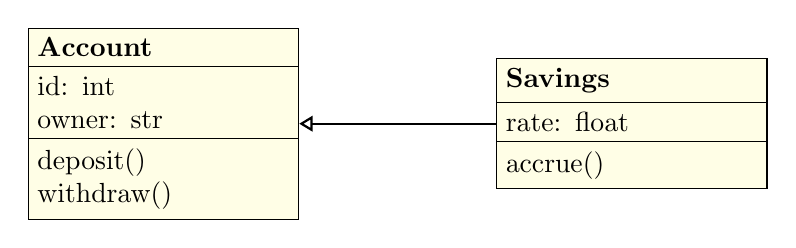
\begin{tikzpicture}[node distance=2.5cm,
      class/.style={draw, rectangle split, rectangle split parts=3, fill=yellow!10, align=left,
        text width=3.2cm}]
    \node[class] (a) {\textbf{Account}
      \nodepart{second} id: int\\ owner: str
      \nodepart{third} deposit()\\ withdraw()};
    \node[class, right=of a] (b) {\textbf{Savings}
      \nodepart{second} rate: float
      \nodepart{third} accrue()};
    \draw[-{Triangle[open]}, thick] (b) -- (a);
  \end{tikzpicture}
\end{frame}

\begin{frame}{Nodes with drop shadows}
  \centering
  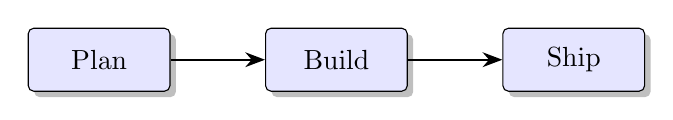
\begin{tikzpicture}[node distance=1.2cm, sh/.style={box, drop shadow}]
    \node[sh] (a) {Plan};
    \node[sh, right=of a] (b) {Build};
    \node[sh, right=of b] (c) {Ship};
    \draw[arr] (a) -- (b);
    \draw[arr] (b) -- (c);
  \end{tikzpicture}
\end{frame}

\begin{frame}{Nodes with shaded fills}
  \centering
  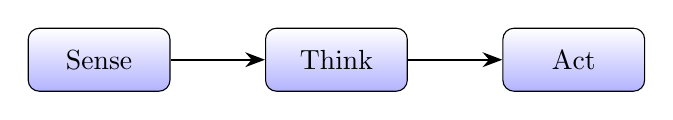
\begin{tikzpicture}[node distance=1.2cm,
      sh/.style={draw, rounded corners, top color=white, bottom color=blue!30, minimum width=1.8cm,
        minimum height=0.8cm}]
    \node[sh] (a) {Sense};
    \node[sh, right=of a] (b) {Think};
    \node[sh, right=of b] (c) {Act};
    \draw[arr] (a) -- (b);
    \draw[arr] (b) -- (c);
  \end{tikzpicture}
\end{frame}

\begin{frame}{Labels with math and subscripts}
  \centering
  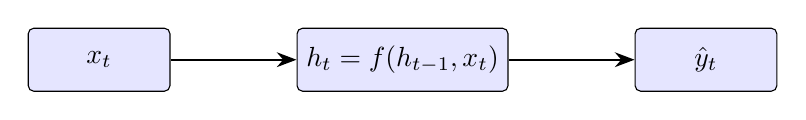
\begin{tikzpicture}[node distance=1.6cm]
    \node[box] (a) {$x_t$};
    \node[box, right=of a] (b) {$h_t = f(h_{t-1}, x_t)$};
    \node[box, right=of b] (c) {$\hat y_t$};
    \draw[arr] (a) -- (b);
    \draw[arr] (b) -- (c);
  \end{tikzpicture}
\end{frame}

% --- Grouping ---------------------------------------------------------------------------------

\begin{frame}{A dashed container around nodes (fit)}
  \centering
  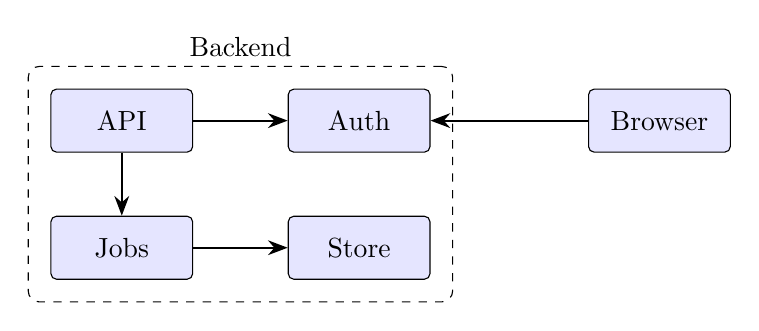
\begin{tikzpicture}[node distance=0.8cm and 1.2cm]
    \node[box] (a) {API};
    \node[box, right=of a] (b) {Auth};
    \node[box, below=of a] (c) {Jobs};
    \node[box, right=of c] (d) {Store};
    \node[box, right=2cm of b] (e) {Browser};
    \draw[arr] (a) -- (b);
    \draw[arr] (a) -- (c);
    \draw[arr] (c) -- (d);
    \draw[arr] (e) -- (b);
    \begin{scope}[on background layer]
      \node[draw, dashed, rounded corners, fit=(a)(b)(c)(d), inner sep=8pt, label=above:Backend] {};
    \end{scope}
  \end{tikzpicture}
\end{frame}

\begin{frame}{Filled background regions behind groups}
  \centering
  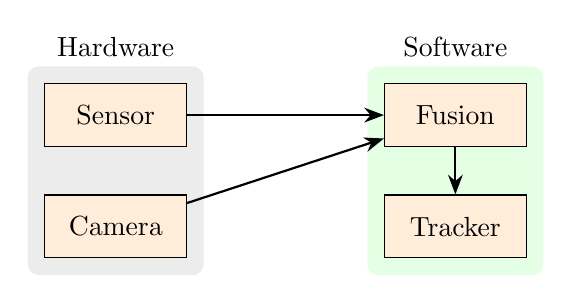
\begin{tikzpicture}[node distance=0.6cm and 1cm]
    \node[sq] (a) {Sensor};
    \node[sq, below=of a] (b) {Camera};
    \node[sq, right=2.5cm of a] (c) {Fusion};
    \node[sq, below=of c] (d) {Tracker};
    \draw[arr] (a) -- (c);
    \draw[arr] (b) -- (c);
    \draw[arr] (c) -- (d);
    \begin{scope}[on background layer]
      \node[fill=gray!15, rounded corners, fit=(a)(b), inner sep=6pt] (g1) {};
      \node[fill=green!10, rounded corners, fit=(c)(d), inner sep=6pt] (g2) {};
    \end{scope}
    \node[above] at (g1.north) {Hardware};
    \node[above] at (g2.north) {Software};
  \end{tikzpicture}
\end{frame}

\begin{frame}{Layered architecture stack}
  \centering
  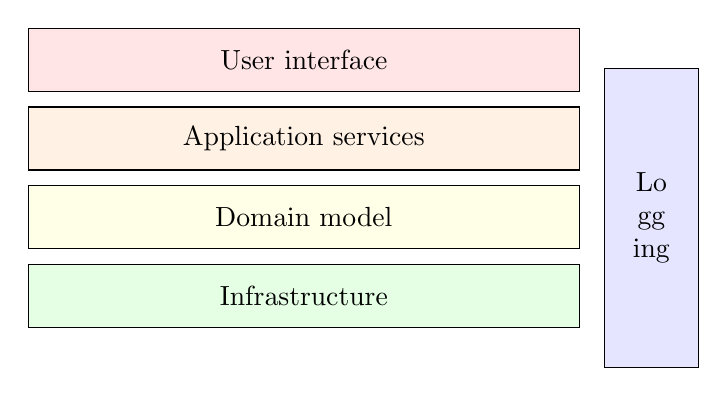
\begin{tikzpicture}
    \node[layer=red!10] (ui) at (0,3) {User interface};
    \node[layer=orange!10] (app) at (0,2) {Application services};
    \node[layer=yellow!10] (dom) at (0,1) {Domain model};
    \node[layer=green!10] (inf) at (0,0) {Infrastructure};
    \node[draw, fill=blue!10, minimum height=3.8cm, minimum width=1.2cm, right=0.3cm of app.east,
      anchor=north west, yshift=0.9cm, align=center] (x) {Lo\\gg\\ing};
  \end{tikzpicture}
\end{frame}

% --- Graphs -----------------------------------------------------------------------------------

\begin{frame}{A tree with straight edges}
  \centering
  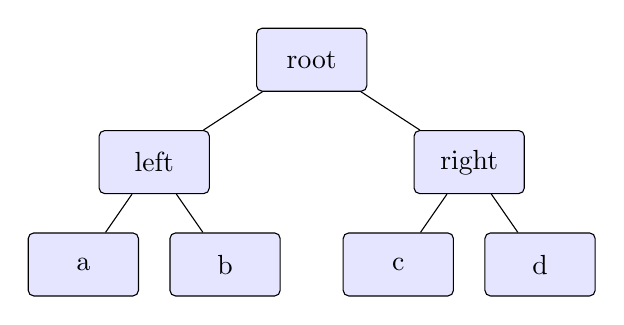
\begin{tikzpicture}[level distance=1.3cm,
      level 1/.style={sibling distance=4cm}, level 2/.style={sibling distance=1.8cm},
      every node/.style={box, minimum width=1.4cm}]
    \node {root}
      child {node {left} child {node {a}} child {node {b}}}
      child {node {right} child {node {c}} child {node {d}}};
  \end{tikzpicture}
\end{frame}

\begin{frame}{An org chart with elbow edges}
  \centering
  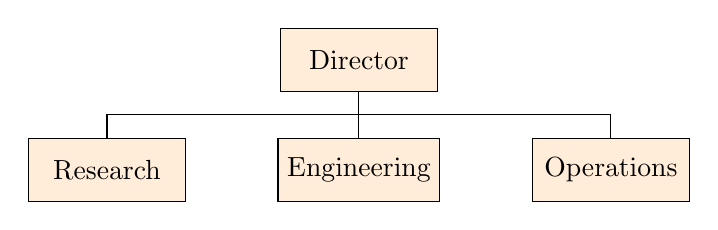
\begin{tikzpicture}[level distance=1.4cm,
      level 1/.style={sibling distance=3.2cm},
      edge from parent fork down,
      every node/.style={sq, minimum width=2cm}]
    \node {Director}
      child {node {Research}}
      child {node {Engineering}}
      child {node {Operations}};
  \end{tikzpicture}
\end{frame}

\begin{frame}{A neural network}
  \centering
  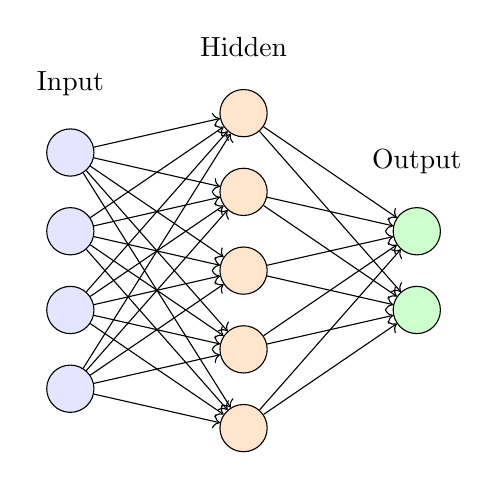
\begin{tikzpicture}[x=2.2cm, y=1cm, n/.style={draw, circle, fill=blue!10, minimum size=0.6cm}]
    \foreach \i in {1,...,4} \node[n] (i\i) at (0,-\i) {};
    \foreach \i in {1,...,5} \node[n, fill=orange!20] (h\i) at (1,-\i+0.5) {};
    \foreach \i in {1,...,2} \node[n, fill=green!20] (o\i) at (2,-\i-1) {};
    \foreach \i in {1,...,4} \foreach \j in {1,...,5} \draw[->] (i\i) -- (h\j);
    \foreach \i in {1,...,5} \foreach \j in {1,...,2} \draw[->] (h\i) -- (o\j);
    \node[above] at (0,-0.4) {Input};
    \node[above] at (1,0.1) {Hidden};
    \node[above] at (2,-1.4) {Output};
  \end{tikzpicture}
\end{frame}

\begin{frame}{A state machine (automata)}
  \centering
  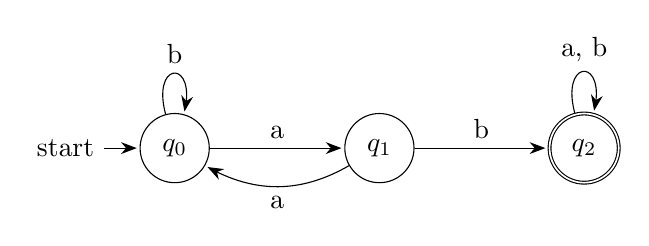
\begin{tikzpicture}[shorten >=1pt, node distance=2.6cm, on grid, auto, >={Stealth[length=2mm]}]
    \node[state, initial] (q0) {$q_0$};
    \node[state] (q1) [right=of q0] {$q_1$};
    \node[state, accepting] (q2) [right=of q1] {$q_2$};
    \path[->]
      (q0) edge node {a} (q1)
           edge [loop above] node {b} ()
      (q1) edge node {b} (q2)
           edge [bend left] node {a} (q0)
      (q2) edge [loop above] node {a, b} ();
  \end{tikzpicture}
\end{frame}

\begin{frame}{A state machine with word labels}
  \centering
  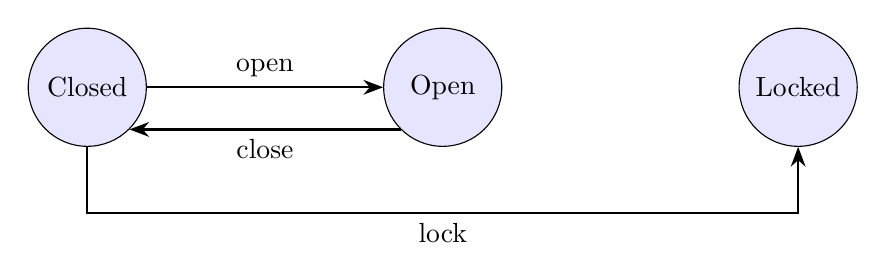
\begin{tikzpicture}[node distance=3cm, st/.style={draw, circle, fill=blue!10, minimum size=1.5cm}]
    \node[st] (a) {Closed};
    \node[st, right=of a] (b) {Open};
    \node[st, right=of b] (c) {Locked};
    \draw[arr] (a) -- node[above] {open} (b);
    \draw[arr] (b.south west) -- node[below] {close} (a.south east);
    \draw[arr] (a) -- ++(0,-1.6) -| node[pos=0.25, below] {lock} (c);
  \end{tikzpicture}
\end{frame}

\begin{frame}[fragile]{A matrix of nodes with arrows}
  \centering
  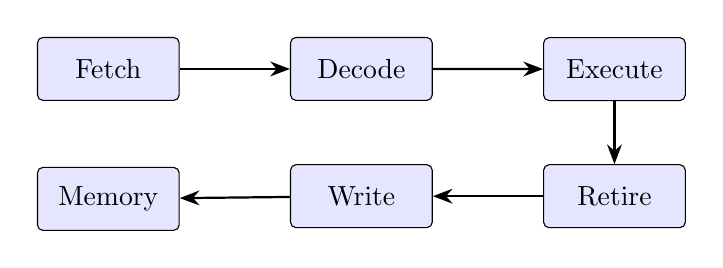
\begin{tikzpicture}
    \matrix (m) [matrix of nodes, row sep=0.8cm, column sep=1.4cm,
      nodes={box, minimum width=1.8cm}] {
      Fetch  & Decode & Execute \\
      Memory & Write  & Retire  \\
    };
    \draw[arr] (m-1-1) -- (m-1-2);
    \draw[arr] (m-1-2) -- (m-1-3);
    \draw[arr] (m-1-3) -- (m-2-3);
    \draw[arr] (m-2-3) -- (m-2-2);
    \draw[arr] (m-2-2) -- (m-2-1);
  \end{tikzpicture}
\end{frame}

\begin{frame}{A chain with a fork and a join}
  \centering
  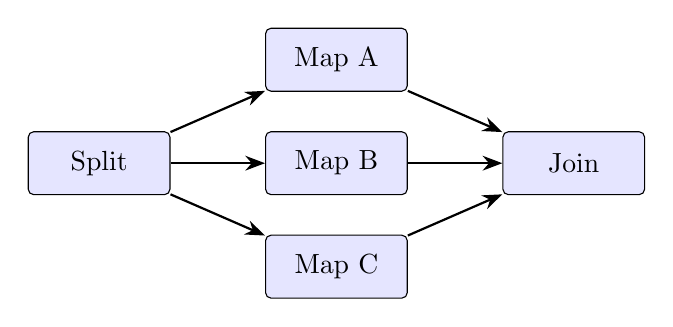
\begin{tikzpicture}[node distance=0.5cm and 1.2cm]
    \node[box] (s) {Split};
    \node[box, above right=of s] (a) {Map A};
    \node[box, right=of s] (b) {Map B};
    \node[box, below right=of s] (c) {Map C};
    \node[box, right=of b] (j) {Join};
    \foreach \x in {a,b,c} { \draw[arr] (s) -- (\x); \draw[arr] (\x) -- (j); }
  \end{tikzpicture}
\end{frame}

\begin{frame}{A sequence diagram}
  \centering
  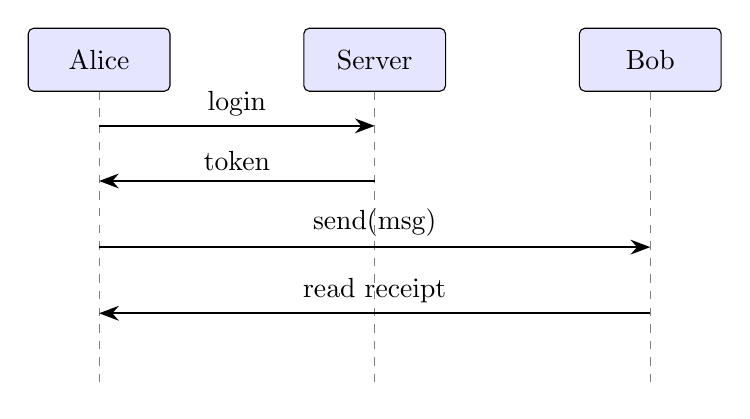
\begin{tikzpicture}[y=0.7cm]
    \foreach \x/\n in {0/Alice, 3.5/Server, 7/Bob} {
      \node[box] (\n) at (\x,0) {\n};
      \draw[dashed, gray] (\n.south) -- (\x,-6);
    }
    \draw[arr] (0,-1.2) -- node[above] {login} (3.5,-1.2);
    \draw[arr] (3.5,-2.2) -- node[above] {token} (0,-2.2);
    \draw[arr] (0,-3.4) -- node[above] {send(msg)} (7,-3.4);
    \draw[arr] (7,-4.6) -- node[above] {read receipt} (0,-4.6);
  \end{tikzpicture}
\end{frame}

\begin{frame}{A timeline with ticks and events}
  \centering
  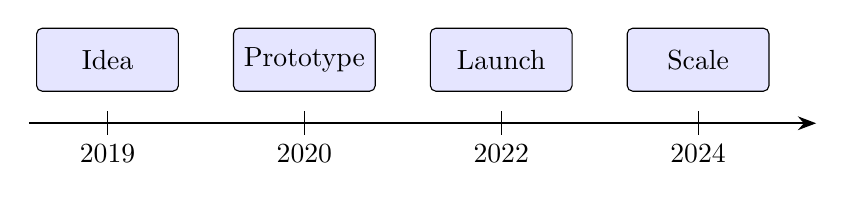
\begin{tikzpicture}
    \draw[thick, -{Stealth}] (0,0) -- (10,0);
    \foreach \x/\y in {1/2019, 3.5/2020, 6/2022, 8.5/2024} {
      \draw (\x,0.15) -- (\x,-0.15) node[below] {\y};
    }
    \node[box, above=0.4cm] at (1,0) {Idea};
    \node[box, above=0.4cm] at (3.5,0) {Prototype};
    \node[box, above=0.4cm] at (6,0) {Launch};
    \node[box, above=0.4cm] at (8.5,0) {Scale};
  \end{tikzpicture}
\end{frame}

\begin{frame}{A brace over a group of steps}
  \centering
  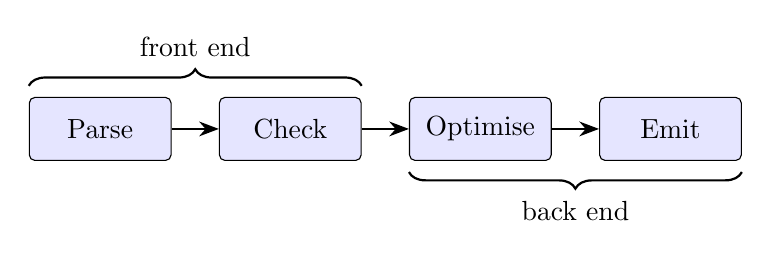
\begin{tikzpicture}[node distance=0.6cm]
    \node[box] (a) {Parse};
    \node[box, right=of a] (b) {Check};
    \node[box, right=of b] (c) {Optimise};
    \node[box, right=of c] (d) {Emit};
    \draw[arr] (a) -- (b);
    \draw[arr] (b) -- (c);
    \draw[arr] (c) -- (d);
    \draw[decorate, decoration={brace, amplitude=6pt}, thick]
      ([yshift=4pt]a.north west) -- node[above=7pt] {front end} ([yshift=4pt]b.north east);
    \draw[decorate, decoration={brace, amplitude=6pt, mirror}, thick]
      ([yshift=-4pt]c.south west) -- node[below=7pt] {back end} ([yshift=-4pt]d.south east);
  \end{tikzpicture}
\end{frame}

\begin{frame}{A Venn diagram}
  \centering
  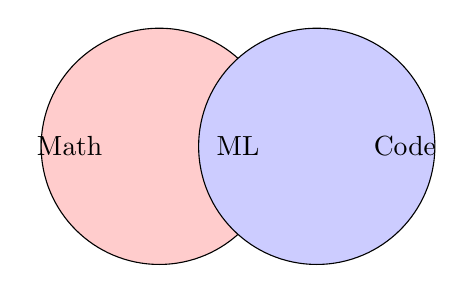
\begin{tikzpicture}
    \draw[fill=red!20] (0,0) circle (1.5cm) node[left=0.6cm] {Math};
    \draw[fill=blue!20] (2,0) circle (1.5cm) node[right=0.6cm] {Code};
    \node at (1,0) {ML};
  \end{tikzpicture}
\end{frame}

\begin{frame}{A mind map}
  \centering
  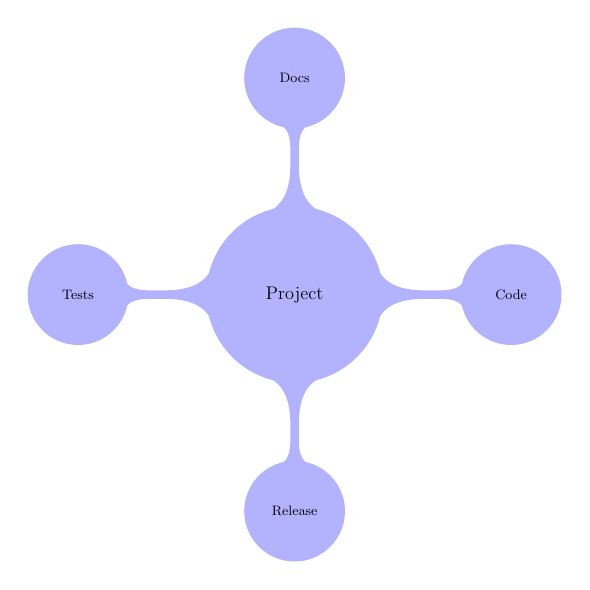
\begin{tikzpicture}[mindmap, concept color=blue!30, every node/.style={concept}, scale=0.55,
      transform shape]
    \node {Project}
      child[grow=0] {node {Code}}
      child[grow=90] {node {Docs}}
      child[grow=180] {node {Tests}}
      child[grow=270] {node {Release}};
  \end{tikzpicture}
\end{frame}

\begin{frame}[fragile]{A commutative diagram (tikz-cd)}
  \centering
  \begin{tikzcd}[column sep=large, row sep=large]
    A \arrow[r, "f"] \arrow[d, "g"'] & B \arrow[d, "h"] \\
    C \arrow[r, "k"'] & D
  \end{tikzcd}
\end{frame}

\begin{frame}{A circuit (circuitikz)}
  \centering
  \begin{circuitikz}
    \draw (0,0) to[battery1, l=$V$] (0,3)
      to[R, l=$R_1$] (4,3)
      to[C, l=$C_1$] (4,0) -- (0,0);
    \draw (4,3) -- (6,3) to[L, l=$L_1$] (6,0) -- (4,0);
  \end{circuitikz}
\end{frame}

\begin{frame}{A control loop block diagram}
  \centering
  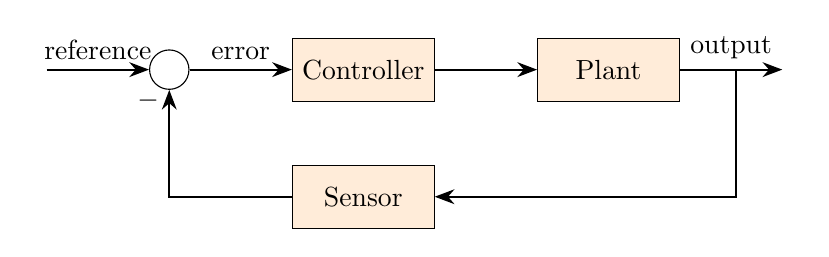
\begin{tikzpicture}[node distance=1.3cm,
      sum/.style={draw, circle, minimum size=0.5cm, inner sep=0pt}]
    \node (in) {};
    \node[sum, right=of in] (s) {};
    \node[sq, right=of s] (c) {Controller};
    \node[sq, right=of c] (p) {Plant};
    \node[right=of p] (out) {};
    \node[sq, below=0.8cm of c] (m) {Sensor};
    \draw[arr] (in) -- node[above] {reference} (s);
    \draw[arr] (s) -- node[above] {error} (c);
    \draw[arr] (c) -- (p);
    \draw[arr] (p) -- node[above] {output} (out);
    \draw[arr] ($(p.east)!0.5!(out)$) |- (m);
    \draw[arr] (m) -| node[pos=0.95, left] {$-$} (s);
  \end{tikzpicture}
\end{frame}

% --- Steps --------------------------------------------------------------------------------------

\begin{frame}{Nodes revealed step by step}
  \centering
  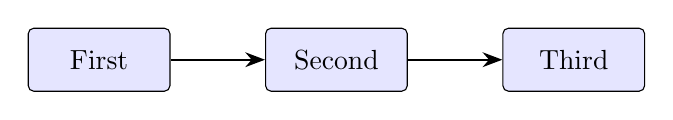
\begin{tikzpicture}[node distance=1.2cm]
    \node[box] (a) {First};
    \node<2->[box, right=of a] (b) {Second};
    \node<3->[box, right=of b] (c) {Third};
    \draw<2->[arr] (a) -- (b);
    \draw<3->[arr] (b) -- (c);
  \end{tikzpicture}
\end{frame}

\begin{frame}{A system architecture}
  \centering
  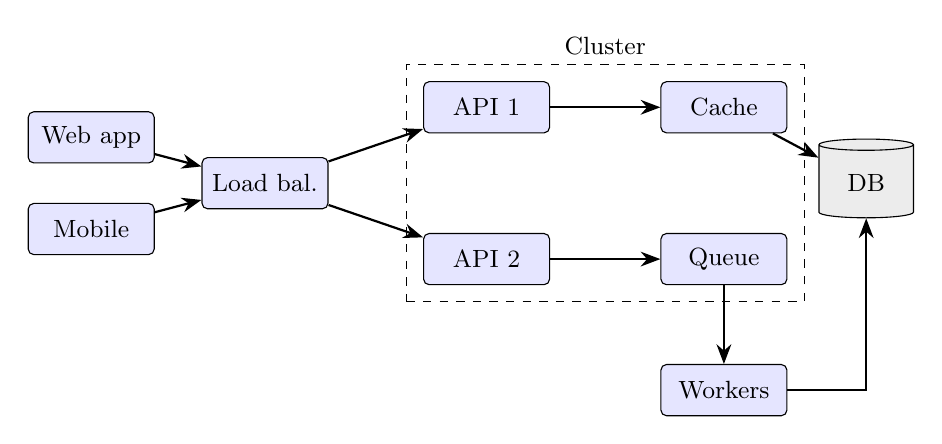
\begin{tikzpicture}[node distance=0.5cm and 0.9cm, font=\small,
      s/.style={box, minimum width=1.6cm, minimum height=0.65cm}]
    \node[s] (web) {Web app};
    \node[s, below=of web] (mob) {Mobile};
    \node[s, right=1.4cm of $(web)!0.5!(mob)$] (lb) {Load bal.};
    \node[s, above right=0.3cm and 1.2cm of lb] (api1) {API 1};
    \node[s, below right=0.3cm and 1.2cm of lb] (api2) {API 2};
    \node[s, right=1.4cm of api1] (cache) {Cache};
    \node[s, right=1.4cm of api2] (queue) {Queue};
    \node[draw, cylinder, shape border rotate=90, aspect=0.2, fill=gray!15, minimum height=1cm,
      minimum width=1.2cm, right=1.2cm of $(cache)!0.5!(queue)$] (db) {DB};
    \node[s, below=1cm of queue] (work) {Workers};
    \draw[arr] (web) -- (lb);
    \draw[arr] (mob) -- (lb);
    \draw[arr] (lb) -- (api1);
    \draw[arr] (lb) -- (api2);
    \draw[arr] (api1) -- (cache);
    \draw[arr] (api2) -- (queue);
    \draw[arr] (cache) -- (db);
    \draw[arr] (queue) -- (work);
    \draw[arr] (work) -| (db);
    \begin{scope}[on background layer]
      \node[draw, dashed, fit=(api1)(api2)(cache)(queue), inner sep=6pt, label=above:Cluster] {};
    \end{scope}
  \end{tikzpicture}
\end{frame}

\end{document}
